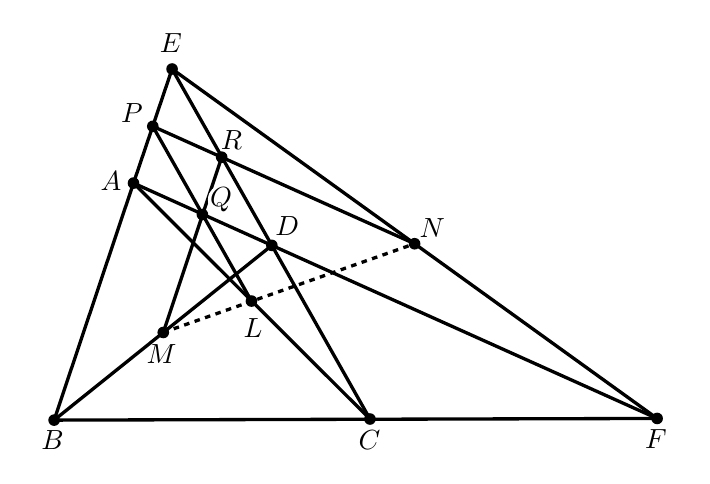
\begin{tikzpicture}[scale = 0.7]
    \clip(-1.74,-0.93) rectangle (10.12,6.84);
    \draw [line width=1.2pt] (-1.26,-0.28)-- (0.18,4.02);
    \draw [line width=1.2pt] (4.47,-0.26)-- (2.69,2.89);
    \draw [line width=1.2pt] (2.69,2.89)-- (0.18,4.02);
    \draw [line width=1.2pt] (-1.26,-0.28)-- (9.68,-0.25);
    \draw [line width=1.2pt] (2.69,2.89)-- (9.68,-0.25);
    \draw [line width=1.2pt] (2.69,2.89)-- (0.88,6.09);
    \draw [line width=1.2pt] (0.18,4.02)-- (0.88,6.09);
    \draw [line width=1.2pt] (0.88,6.09)-- (9.68,-0.25);
    \draw [line width=1.2pt] (-1.26,-0.28)-- (2.69,2.89);
    \draw [line width=1.2pt] (0.18,4.02)-- (4.47,-0.26);
    \draw [line width=1.2pt] (0.53,5.05)-- (2.32,1.88);
    \draw [line width=1.2pt] (1.78,4.49)-- (0.72,1.31);
    \draw [line width=1.2pt] (0.53,5.05)-- (5.28,2.92);
    \draw [line width=1.2pt,dash pattern=on 2pt off 2pt] (0.72,1.31)-- (5.28,2.92);
    \begin{scriptsize}
        \normalsize
        \fill [color=black] (0.18,4.02) circle (3.0pt);
        \draw[color=black] (-0.23,4.06) node {$A$};
        \fill [color=black] (-1.26,-0.28) circle (3.0pt);
        \draw[color=black] (-1.29,-0.65) node {$B$};
        \fill [color=black] (4.47,-0.26) circle (3.0pt);
        \draw[color=black] (4.46,-0.65) node {$C$};
        \fill [color=black] (2.69,2.89) circle (3.0pt);
        \draw[color=black] (2.97,3.24) node {$D$};
        \fill [color=black] (0.88,6.09) circle (3.0pt);
        \draw[color=black] (0.86,6.56) node {$E$};
        \fill [color=black] (9.68,-0.25) circle (3.0pt);
        \draw[color=black] (9.66,-0.63) node {$F$};
        \fill [color=black] (0.72,1.31) circle (3.0pt);
        \draw[color=black] (0.69,0.92) node {$M$};
        \fill [color=black] (2.32,1.88) circle (3.0pt);
        \draw[color=black] (2.35,1.39) node {$L$};
        \fill [color=black] (1.43,3.45) circle (3.0pt);
        \draw[color=black] (1.77,3.72) node[fill = white, rounded corners = 5pt, inner sep=0.8pt] {$Q$};
        \fill [color=black] (0.53,5.05) circle (3.0pt);
        \draw[color=black] (0.15,5.29) node {$P$};
        \fill [color=black] (1.78,4.49) circle (3.0pt);
        \draw[color=black] (1.96,4.81) node[fill = white, rounded corners = 5pt, inner sep=0.8pt] {$R$};
        \fill [color=black] (5.28,2.92) circle (3.0pt);
        \draw[color=black] (5.6,3.2) node {$N$};
    \end{scriptsize}
\end{tikzpicture}